\section{Dense Neural Networks}
\subsection{Deep vs Shallow}
\begin{figure}
    \makebox[\linewidth][c]{%
    \centering
    \begin{subfigure}{.65\textwidth}
        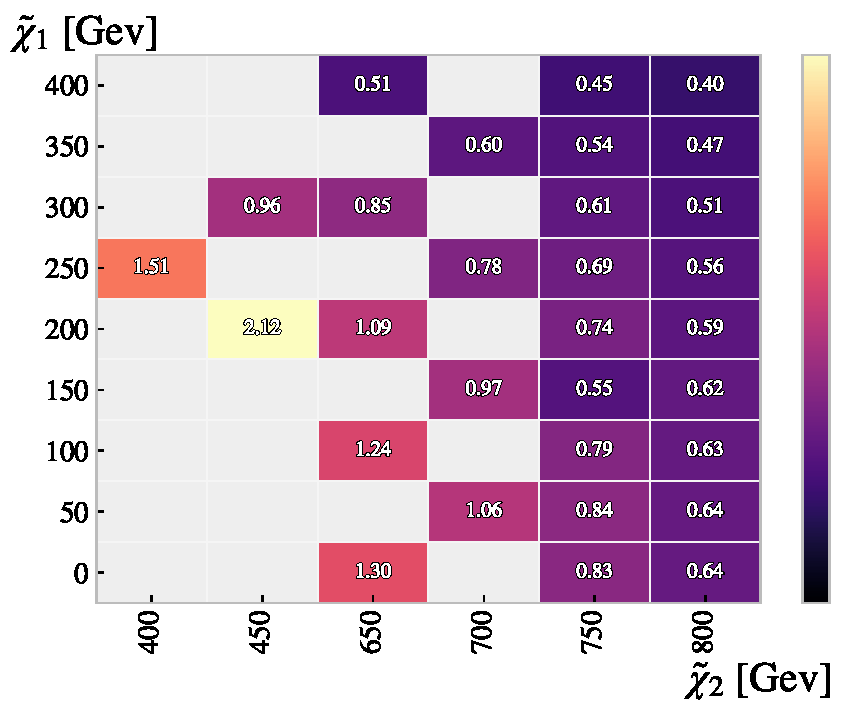
\includegraphics[width=\textwidth]{Figures/MLResults/NN/SUSY/Grid/NNshallowGridSig.pdf}
    \end{subfigure}
    }
    \caption{A grid displaying the achieved significance on the original signal set, using the signal region 
    created by the shallow \ac{NN} network.}
    \label{fig:NNshallowGridSig}
\end{figure}
\begin{figure}
    \makebox[\linewidth][c]{%
    \centering
    \begin{subfigure}{.65\textwidth}
        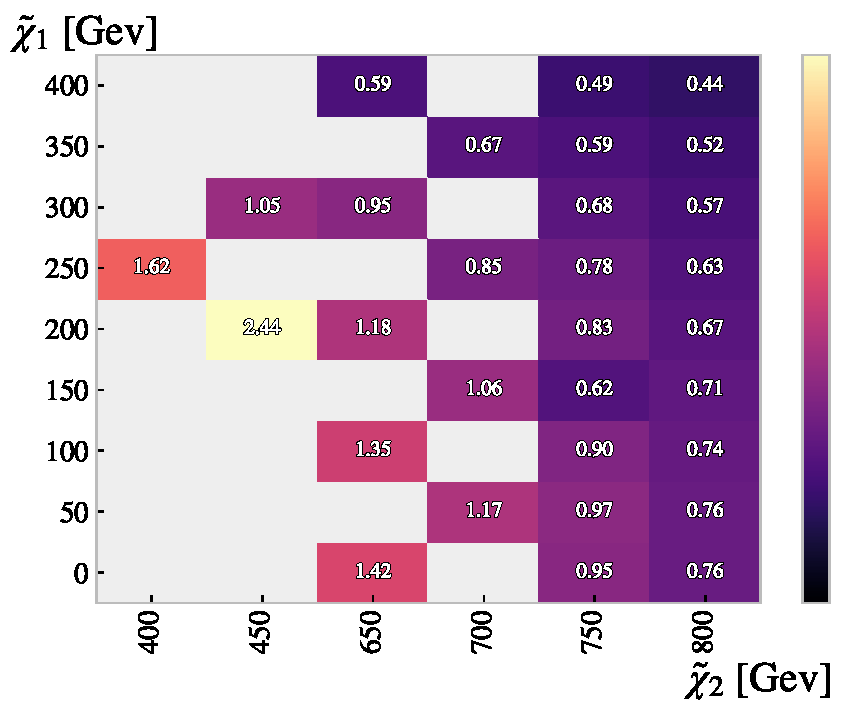
\includegraphics[width=\textwidth]{Figures/MLResults/NN/SUSY/Grid/NNGridSig.pdf}
    \end{subfigure}
    }
    \caption{A grid displaying the achieved significance on the original signal set, using the signal region 
    created by the deep \ac{NN} network.}
    \label{fig:NNGridSig}
\end{figure}
\subsection{Parameter Specific Networks and Interpolation}
As I have touched upon in earlier sections, one possible solution to a diverse signal set is to implement one model for 
each individual signal set.  
\begin{figure}
    \makebox[\linewidth][c]{%
    \centering
    \begin{subfigure}{.6\textwidth}
        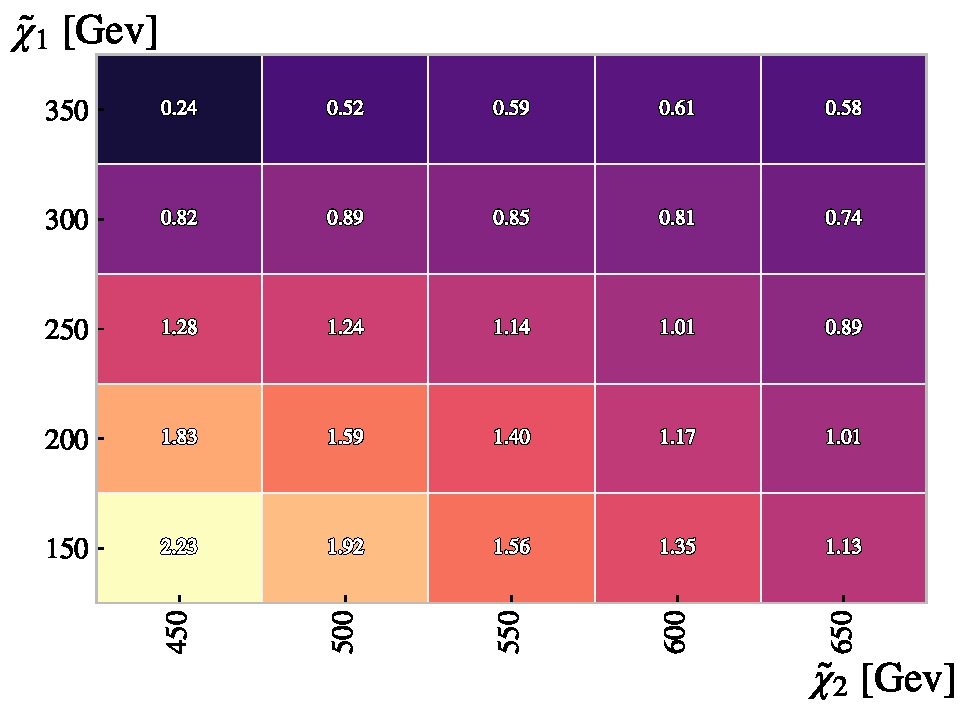
\includegraphics[width=\textwidth]{Figures/MLResults/NN/SUSY/Grid/Interpolation/NN_OneMass_InterpolationGridSig.pdf}
        \caption{}
        \label{fig:OneMass}
    \end{subfigure}
    \hfill
    \begin{subfigure}{.6\textwidth}
        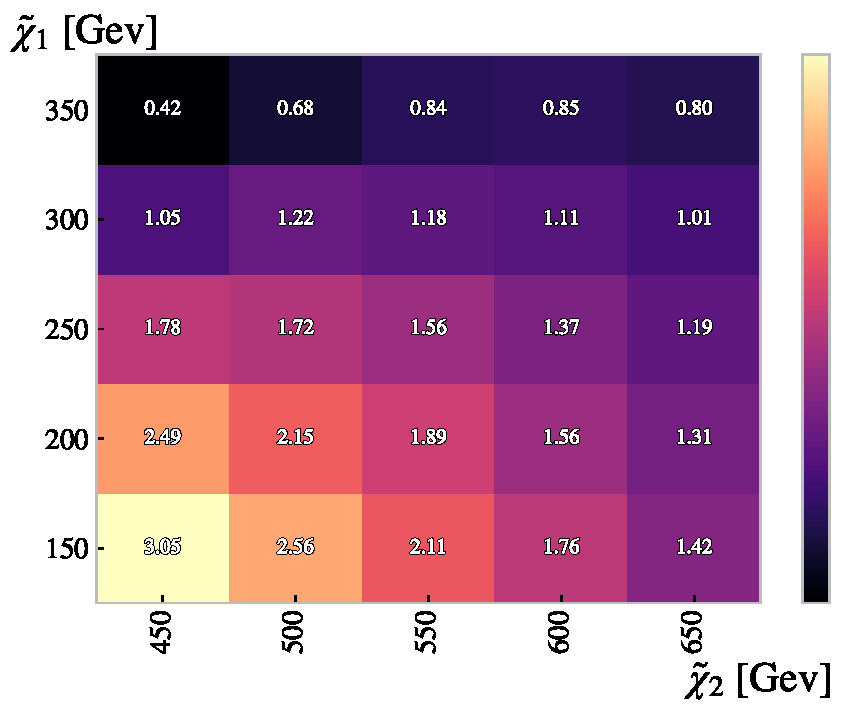
\includegraphics[width=\textwidth]{Figures/MLResults/NN/SUSY/Grid/Interpolation/NN_InterpolationGridSig.pdf}
        \caption{}
        \label{fig:SeveralMass}
    \end{subfigure}
    }
    \caption{}
    \label{fig:Interpolation}
\end{figure}